\documentclass[11pt,a4paper]{article}
\usepackage[a4paper,margin=2.2cm]{geometry}
\usepackage{libertinus}
\usepackage{graphicx}
\usepackage[font=small,labelfont=bf]{caption}
\usepackage{enumitem}
\usepackage{xurl}
\usepackage[hidelinks]{hyperref}
\usepackage{microtype}

\graphicspath{{../figures/out/}}
% Generated by `cpilens report` from results/. Do not edit by hand.
\newcommand{\InScopeWeightEqual}{40.5}
\newcommand{\InScopeWeightNnls}{43.5}
\newcommand{\LLMSpendUSD}{5.62}
\newcommand{\NCorpusTexts}{88{,}622}
\newcommand{\NGoldDouble}{150}
\newcommand{\NGoldSample}{600}
\newcommand{\NGoldStrata}{13}
\newcommand{\NLLMCalls}{9{,}555}
\newcommand{\NLabelsInScope}{28}
\newcommand{\NMocSpecs}{31{,}822}
\newcommand{\NMocTest}{6{,}017}
\newcommand{\NMocTrainval}{25{,}805}
\newcommand{\NOffMarkets}{18}
\newcommand{\NOffProducts}{76{,}269}
\newcommand{\NOffThailand}{10{,}526}
\newcommand{\NOffThailandSilver}{4{,}415}
\newcommand{\NOffThailandThaiScript}{7{,}303}
\newcommand{\NWeakNonthai}{52{,}255}
\newcommand{\NWeakThai}{3{,}945}

\pagestyle{empty}
\setlist{leftmargin=1.2em, itemsep=0.3em, topsep=0.3em}

\begin{document}

{\Large\bfseries How much does product classification cost in basis points?}\par
\vspace{0.3em}
{\large Policy brief: classifying Thai product text for price measurement}\par
\vspace{0.4em}
Thanatchon Chongmankhong\quad\textbullet\quad \today\par
\vspace{0.3em}
{\small\itshape The views expressed are the author's own and do not necessarily reflect those
of the Bank of Thailand. This work uses only publicly available data.}
\vspace{0.8em}

\noindent\textbf{Why it matters.} Prices from retailers' websites and scanner data can make
price measurement faster and more detailed. Before such prices can enter a consumer price
index, every product has to be assigned to an item of the official basket: a bag of jasmine
rice to rice, a carton of UHT milk to milk and dairy products. Done by hand this does not
scale; done by a model it introduces errors. This study asks how large those errors would be
in the unit that matters for policy: basis points (hundredths of a percentage point) of
measured inflation.

\medskip\noindent\textbf{What the study did.} Using only public data, it tested four kinds of
method on Thai product descriptions: low-cost text-matching models, a fine-tuned language
model, two commercial large language models (LLMs) instructed with a few examples, and
``cascades'' that send only the hard cases to an LLM. Each was scored on \NRefSpecs{}
official Thai price-collection descriptions published by the Ministry of Commerce, none of
which was used to train the models built here or to set their thresholds, with every item weighted by its share
of household spending. Each method's mistakes were then fed through a reconstruction of the
Thai CPI to see how far measured inflation would move.

\subsection*{Three findings}

\begin{enumerate}
\item \textbf{The larger LLM classifies almost all of the evaluated basket correctly; low-cost
models do not.} The larger LLM assigned \AccWOpus\% of the evaluated CPI weight to the right
item and the smaller one \AccWHaiku\%. Of the low-cost models given the full descriptions, the best,
the fine-tuned one, reached \AccWXlmrFT\%. A cascade that lets a low-cost model handle the easy cases and sends the rest
to the larger LLM scored \AccWCasEfiveMLPOpus\%, close to the larger LLM on its own, at
\CostPctCasEfiveMLPOpus\% of its cost on the held-out list. All LLM runs
for this study together cost USD~\LLMSpendUSD.

\item \textbf{With the larger LLM, classification would move headline inflation by about
\BpYoyRmseHeadlineOpus{} basis points.} That is the typical error of the year-on-year rate over
\NMonthsYoy{} months. Allowing for the fact that errors cluster within groups of similar
products, the error could be up to \BpYoyRmseHeadlineOpusClusterHi{} basis points, and more
under other plausible assumptions about the basket weights; on average it would overstate
inflation slightly (by \BpYoyMeanHeadlineOpus{} basis points). For food inflation the typical
error is \BpYoyRmseFoodOpus{} basis points. The low-cost models misstate headline inflation by
between \BpYoyRmseHeadlineBgeMLP{} and \BpYoyRmseHeadlineEfiveMLP{} basis points; two of them
miss food inflation by \BpYoyRmseFoodXlmrFT{} and \BpYoyRmseFoodEfiveMLP{} basis points, and
one would have understated it in every month.

\item \textbf{Accuracy alone is a poor guide.} Two low-cost models with about the same
accuracy differed several-fold in basis points, because what matters is whether the confused
items' prices moved apart. Most of the LLMs' remaining errors came from two items whose
official contents differ from what their names suggest: the official ``personal items''
include wristwatches, school bags and hair dryers, and margarine is counted with milk and
dairy products, not with oils and fats. Better documentation of the basket may well fix
these; that was not tested.
\end{enumerate}

\begin{figure}[h]
\centering
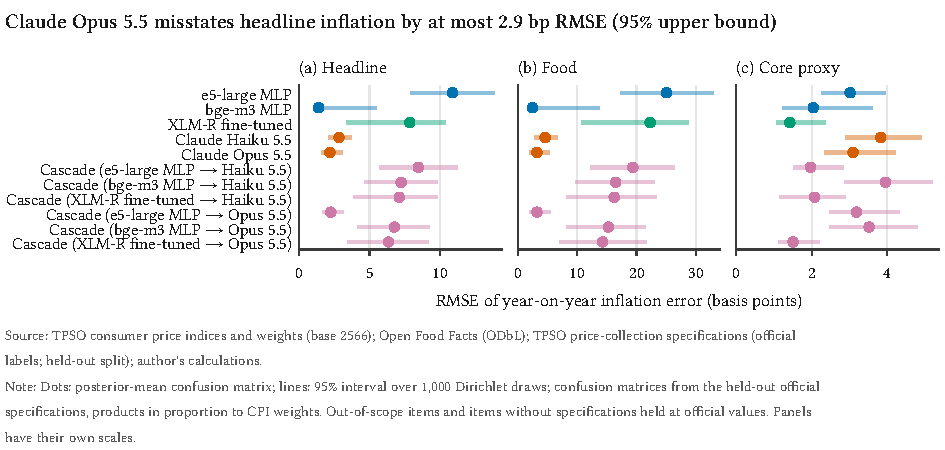
\includegraphics[width=\textwidth]{fig10_bp_error.pdf}
\caption{\textbf{The LLMs and the cascade to the larger LLM would misstate inflation by a few
basis points; low-cost models range from as little to several times more.} Typical error
(RMSE) of year-on-year inflation caused by each method's classification mistakes, over
\NMonthsYoy{} months. Dots: central estimate; thick lines: \CfgCI\% interval treating each
description as independent; thin lines: allowing errors to cluster. On core inflation, which
excludes raw food and energy, the low-cost models do as well as the LLMs. Source: Ministry of
Commerce; Trade Policy and Strategy Office; author's calculations.}
\end{figure}

\subsection*{What it means for central banks in Asia}

\begin{itemize}
\item \textbf{Basis points are a more useful yardstick than accuracy.} The method needs only a
test set of labelled products, the published CPI weights and the published item indices, so
an office could state the classification error of a new data source before using it.
\item \textbf{Published specification lists are valuable.} The Ministry of Commerce's open
specifications made this study possible. Descriptions of what each item includes and
excludes could address the largest errors found here.
\item \textbf{LLMs are affordable at this scale; governance is the larger question.}
Commercial models change over time, so responses would need to be stored and versioned.
Open-weight models that an office could run itself were not tested.
\item \textbf{Languages with few labelled data can start from other languages.} With no Thai
training labels at all, a low-cost model trained on products in other languages placed
\AccWEfiveMLPZeroShot\% of the weight correctly: a starting point, not a result an index can
rely on.
\end{itemize}

\subsection*{Caveats}

The test descriptions are the statistical office's own short texts; shop descriptions are
longer and noisier, and accuracy on them will be lower. The descriptions are public, so the
LLMs may have seen them in training. Item weights below the published groups are estimated,
and the results depend on how. The basis-point figures assume a mix of products in
proportion to household spending, cover the \RefWeightEqual\% of the headline weight that the
test set can evaluate, and measure classification error only, not the other errors of a
web-price index. A low basis-point error is meaningful only together with high accuracy: a
model that classifies little of the basket also moves the index little. The results are for
one country and one point in time and are not directly comparable with studies of other
markets. The two LLMs are \NameOpus{} (larger) and \NameHaiku{} (smaller).

\vspace{0.5em}
{\small\noindent Full paper, code and data:
\url{https://github.com/thanatchon36/cpilens} (DOI \href{https://doi.org/10.5281/zenodo.23686886}{10.5281/zenodo.23686886}).} % numbers-ok: DOI

\end{document}
